\documentclass[a4paper,10pt]{article}
\usepackage[utf8]{inputenc}
\usepackage[a4paper,
            bindingoffset=0.2in,
            left=1in,
            right=1in,
            top=1in,
            bottom=1in,
            footskip=.25in]{geometry}

%###############################################################################

%\input{~/layout/global_layout}


%###############################################################################

% packages begin

\usepackage[
  backend=biber,
  sortcites=true,
  style=alphabetic,
  eprint=true,
  backref=true
]{biblatex}
\addbibresource{bibliographie.bib}
\usepackage[acronym]{glossaries}

\usepackage{euscript}[mathcal]
% e.g. \mathcal{A} for fancy letters in mathmode
\usepackage{amsmath,amssymb,amstext,amsthm}

\usepackage{mdframed}
\newmdtheoremenv[nobreak=true]{problem}{Problem}[subsection]
\newmdtheoremenv[nobreak=true]{claim}{Claim}[subsection]
\newtheorem{definition}{Definition}[subsection]
\newtheorem{lemma}{Lemma}[claim]
\newtheorem{plemma}{Lemma}[problem]

\usepackage{mathtools}
\DeclarePairedDelimiter\ceil{\lceil}{\rceil}
\DeclarePairedDelimiter\floor{\lfloor}{\rfloor}

\usepackage{enumerate}
\usepackage[pdftex]{graphicx}
\usepackage{subcaption}
% 'draft' für schnelleres rendern mitübergeben -> [pdftex, draft]
% dadruch wird nicht das bild mitgerendered, sondern nur ein kasten mit bildname -> schont ressourcen

\usepackage{hyperref}

\usepackage{tikz}
\usetikzlibrary{arrows,automata,matrix,positioning,shapes}

% for adding non-formatted text to include source-code
\usepackage{listings}
\lstset{language=Python,basicstyle=\footnotesize}
% z.B.:
% \lstinputlisting{source_filename.py}
% \lstinputlisting[lanugage=Python, firstline=37, lastline=45]{source_filename.py}
%
% oder
%
% \begin{lstlisting}[frame=single]
% CODE HERE
%\end{lstlisting}
\usepackage{algorithm}
\usepackage{algpseudocode}

\usepackage{wasysym}

\usepackage{titling}
\usepackage{titlesec}
\usepackage[nocheck]{fancyhdr}
\usepackage{lastpage}

\usepackage{kantlipsum}
\usepackage[colorinlistoftodos,prependcaption,textsize=tiny]{todonotes}

% packages end
%###############################################################################

\pretitle{% add some rules
  \begin{center}
    \LARGE\bfseries
} %, make the fonts bigger, make the title (only) bold
\posttitle{%
  \end{center}%
  %\vskip .75em plus .25em minus .25em% increase the vertical spacing a bit, make this particular glue stretchier
}
\predate{%
  \begin{center}
    \normalsize
}
\postdate{%
  \end{center}%
}

\titleformat*{\section}{\Large\bfseries}
\titleformat*{\subsection}{\large\bfseries}
\titleformat*{\subsubsection}{\normalsize\bfseries}

\titleformat*{\paragraph}{\Large\bfseries}
\titleformat*{\subparagraph}{\large\bfseries}

%###############################################################################

\pagestyle{fancy}
\fancyhf{}
% l=left, c=center, r=right; e=even_pagenumber, o=odd_pagenumber; h=header, f=footer
% example: [lh] -> left header, [lof,ref] -> fotter left when odd, right when even
%\fancyhf[lh]{}
%\fancyhf[ch]{}
%\fancyhf[rh]{}
%\fancyhf[lf]{}
\fancyhf[cf]{\footnotesize Page \thepage\ of \pageref*{LastPage}}
%\fancyhf[rf]{}
\renewcommand{\headrule}{} % removes horizontal header line

% Fotter options for first page

\fancypagestyle{firstpagestyle}{
  \renewcommand{\thedate}{\textmd{}} % removes horizontal header line
  \fancyhf{}
  \fancyhf[lh]{\ttfamily M.Sc. Computer Science\\KTH Royal Institute of Technology}
  \fancyhf[rh]{\ttfamily Period 4\\\today}
  \fancyfoot[C]{\footnotesize Page \thepage\ of \pageref*{LastPage}}
  \renewcommand{\headrule}{} % removes horizontal header line
}
%###############################################################################

\newcommand\extrafootertext[1]{%
    \bgroup
    \renewcommand\thefootnote{\fnsymbol{footnote}}%
    \renewcommand\thempfootnote{\fnsymbol{mpfootnote}}%
    \footnotetext[0]{#1}%
    \egroup
}

%###############################################################################

\title{
  \normalsize{DD2356 VT25 Methods in}\\
  \normalsize{High Performance Computing}\\
  \large{Assignment 1}
}
\author{
  \small Rishi Vijayvargiya\textsuperscript{\textdagger}\\[-0.75ex]
%  \footnotesize\texttt{MN: }\\[-1ex]
  \scriptsize\texttt{rishiv@kth.se}
  \and
  \small Paul Mayer\textsuperscript{\textdagger}\\[-0.75ex]
%  \footnotesize\texttt{MN: }\\[-1ex]
  \scriptsize\texttt{pmayer@kth.se}
  \and
  \small Lennard Herud\textsuperscript{\textdagger}\\[-0.75ex]
%  \footnotesize\texttt{MN: }\\[-1ex]
  \scriptsize\texttt{herud@kth.se}
}
\date{}

%###############################################################################
% define Commands

\newcommand{\N}{\mathbb{N}}
\newcommand{\R}{\mathbb{R}}
\newcommand{\Z}{\mathbb{Z}}
\newcommand{\I}{\mathbb{I}}

\newcommand{\E}{\mathbb{E}}
\newcommand{\Prob}{\mathbb{P}}

\renewcommand{\epsilon}{\varepsilon}

%###############################################################################
\makeatletter
\renewcommand*{\@fnsymbol}[1]{\ensuremath{\ifcase#1\or \dagger\or \ddagger\or
   \mathsection\or \mathparagraph\or \|\or **\or \dagger\dagger
   \or \ddagger\ddagger \else\@ctrerr\fi}}
\makeatother
%###############################################################################

\begin{document}
\maketitle
\extrafootertext{\textsuperscript{\textdagger}Authors made equal contribution to the assignment}
\thispagestyle{firstpagestyle}

\listoftodos
\vspace{1em}

% content begin
%

\section*{Prefix}
The code for our project can be found at this location: \url{https://github.com/paulmyr/DD2356-MethodsHPC/tree/master/1_dardel_simple_benchmarking/code}.

% \tableofcontents
% \newpage

\section{Compiling and Running on Dardel}
\verb|salloc -t 00:30:00 --nodes 1 --ntasks-per-node 128 --cpus-per-task 1 -A edu25.DD2356 -p shared|
\verb|srun -n 128 ./mpi_hello_world.out > log_dd2356_e1_i|

\section{Sustainability and Supercomputers}
\todo[inline]{Exercise 2}

\section{The Memory Mountain}
  We ran the script on dardel.
  We inquired that dardel uses the AMD EPYC™ 7742 cpus.
  This implies the following cache sizes:
  \begin{itemize}
  \item L1: 96 KB(per core), 
  \item L2: 512 KB(per core),
  \item L3: 256 MB(shared)
  \end{itemize}
  The results\footnote{Results found \href{https://github.com/paulmyr/DD2356-MethodsHPC/blob/master/1\_dardel\_simple\_benchmarking/misc/results.txt}{here}.} are visualised in Figure \ref{fig:mem_mountain}.
  \begin{figure}[H]
    \centering
    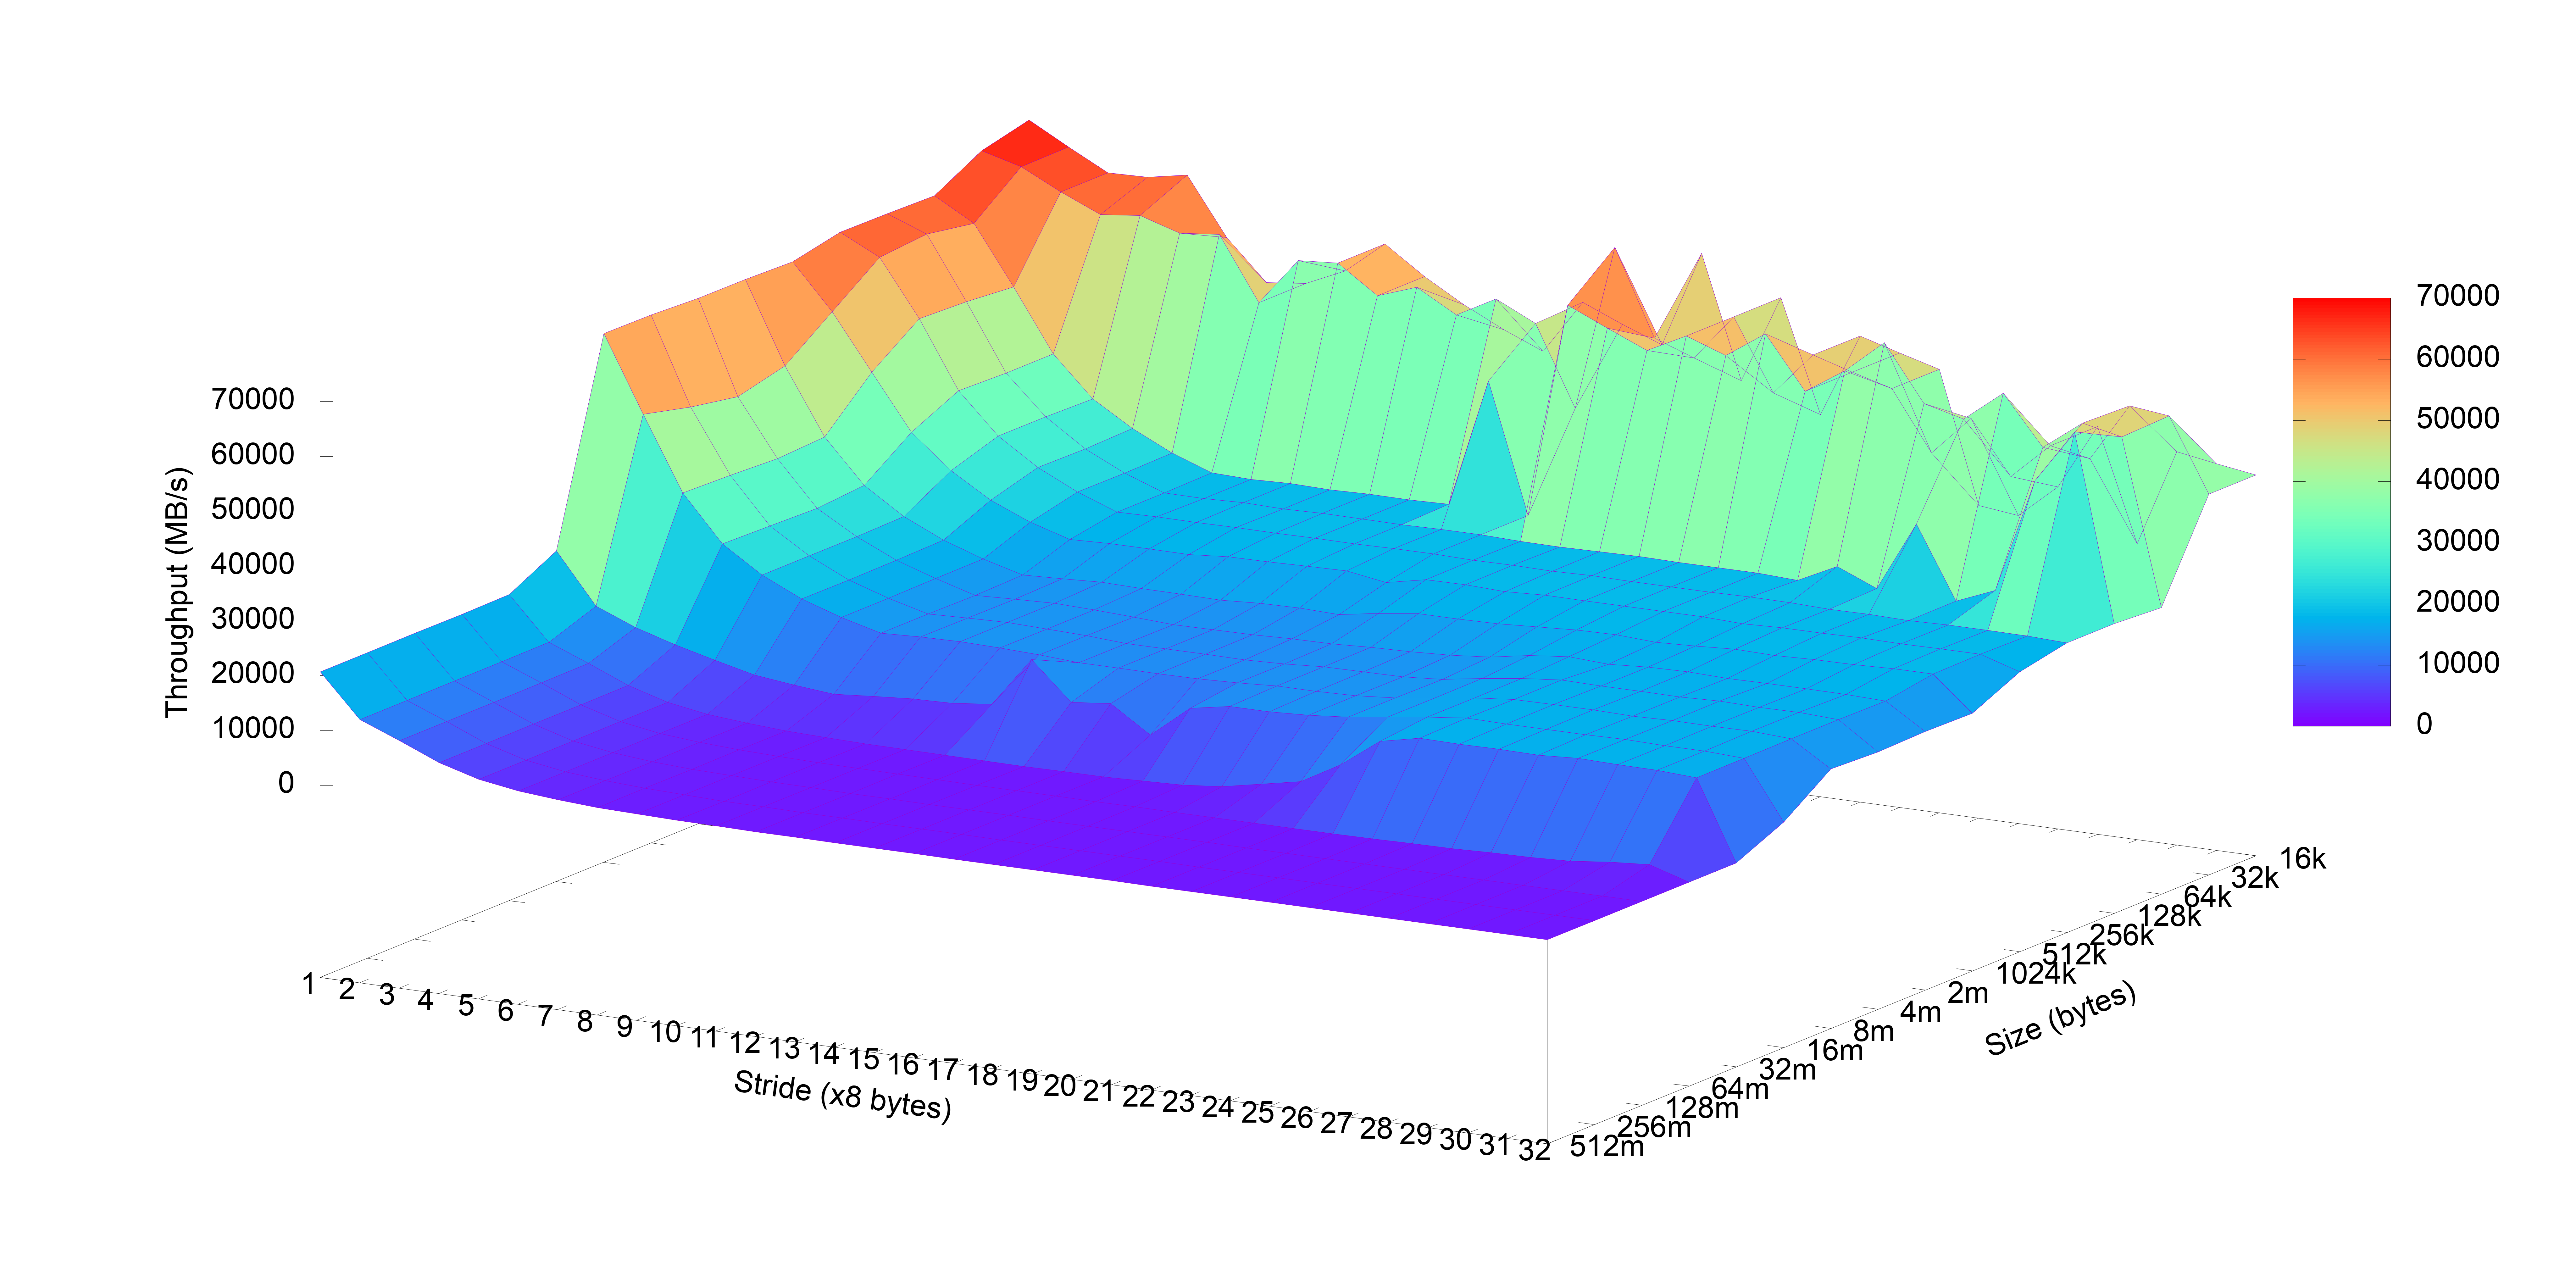
\includegraphics[width=0.9\textwidth]{images/memory_mountain}
    \caption{Memory Mountain Plot}
    \label{fig:mem_mountain}
  \end{figure}
  It clearly shows that the smaller stride and array sizes are, the higher the throughput.
  Inversly the same holds true.
  The bigger the strides and array sizes are, the worse the throughput becomes.
  Suprisingly, for big array sizes (e.g. 512 MB), a stride size of 1 still produces high throughput, even tho the array size surpasses the L3 cache size.

  This has to do with prefetching.
  Prefetching refers to the technique of fetching data that might be used in the near future based in faster memory before it is actually used for the computation.
  This greatly increases performance mainly because fetching data from memory is magnitudes slower than performing arithmetic operations in the processing unit.
  The cpu tries to pre fetch data based on spatial locality, meaning data stored close to the referenced data.
  Spatial Locality means that all those instructions that are stored nearby to the recently executed instruction have a high chance of execution
  It refers to the use of data elements(instructions) that are relatively close in storage locations.
  Spatial locality describes that there is an increased likelyhood that data stored spatially close to recently fetched data is referenced in the near future.
  Many computations perform computations on Lists, Fields or Meshes.
  This means that computations have to be performed on multiple elements typically stored close to each other.
  That is the main reason why increasing the stride reduces spatial locality.
  All of a sudden, elements that are not stored together need to be fetched after each other.
  With a stride size of 1 however, the cpu is able to guess corretly with very high probability, boosting the performance even tho the array size increases the L3 cache size.

  Temporal locality on the other hand describes that data stored at a certain location has an increased likelyhood of beeing fetched again after having been referenced once.
  The main reason for this is that most of heavy computations perform operations in loops, and most of the times is performed on the same data (or data stored in the same location).
  This especially holds true if the data is within a small multiple of the cache size.
  However, for very large data arrays, it might take multiple fetching cylces until the same data location is referenced again, therefore will decrease the temperal locality.
   
 % content end
 %###############################################################################
 
 % \printbibliography
 
 \end{document}
